\documentclass[unicode,11pt,a4paper,oneside,numbers=endperiod,openany]{scrartcl}
\usepackage{graphicx}
\usepackage{subfig}
\usepackage{float}

\usepackage{ifthen}
\usepackage[utf8]{inputenc}
\usepackage{graphics}
\usepackage{graphicx}
\usepackage{hyperref}

\pagestyle{plain}
\voffset -5mm
\oddsidemargin  0mm
\evensidemargin -11mm
\marginparwidth 2cm
\marginparsep 0pt
\topmargin 0mm
\headheight 0pt
\headsep 0pt
\topskip 0pt        
\textheight 255mm
\textwidth 165mm

\newcommand{\duedate} {}
\newcommand{\setduedate}[1]{%
\renewcommand\duedate {Due date:~ #1}}
\newcommand\isassignment {false}
\newcommand{\setassignment}{\renewcommand\isassignment {true}}
\newcommand{\ifassignment}[1]{\ifthenelse{\boolean{\isassignment}}{#1}{}}
\newcommand{\ifnotassignment}[1]{\ifthenelse{\boolean{\isassignment}}{}{#1}}

\newcommand{\assignmentpolicy}{
\begin{table}[h]
\begin{center}
\scalebox{0.8} {%
\begin{tabular}{|p{0.02cm}p{16cm}|}
\hline
&\\
\multicolumn{2}{|c|}{\Large\textbf{HPC  2022 ---  Submission Instructions}}\\
\multicolumn{2}{|c|}{\large\textbf{(Please, notice that following instructions are mandatory: }}\\
\multicolumn{2}{|c|}{\large\textbf{submissions that don't comply with, won't be considered)}}\\
&\\
\textbullet & Assignments must be submitted to \href{https://www.icorsi.ch/course/view.php?id=14652}{iCorsi} (i.e. in electronic format).\\
\textbullet & Provide both executable package and sources (e.g. C/C++ files, Matlab). 
If you are using libraries, please add them in the file. Sources must be organized in directories called:\\
\multicolumn{2}{|c|}{\textit{Project\_number\_lastname\_firstname}}\\
& and  the  file must be called:\\
\multicolumn{2}{|c|}{\textit{project\_number\_lastname\_firstname.zip}}\\
\multicolumn{2}{|c|}{\textit{project\_number\_lastname\_firstname.pdf}}\\
\textbullet &  The TAs will grade your project by reviewing your project write-up, and looking at the implementation 
                 you attempted, and benchmarking your code's performance.\\

\textbullet & You are allowed to discuss all questions with anyone you like; however: (i) your submission must list anyone you discussed problems with and (ii) you must write up your submission independently.\\
\hline
\end{tabular}
}
\end{center}
\end{table}
}
\newcommand{\punkte}[1]{\hspace{1ex}\emph{\mdseries\hfill(#1~\ifcase#1{Points}\or{Points}\else{Points}\fi)}}


\newcommand\serieheader[6]{
\thispagestyle{empty}%
\begin{flushleft}

\includegraphics[width=0.4\textwidth]{usi_inf.png}
\end{flushleft}
  \noindent%
  {\large\ignorespaces{\textbf{#1}}\hspace{\fill}\ignorespaces{ \textbf{#2}}}\\ \\%
  {\large\ignorespaces #3 \hspace{\fill}\ignorespaces #4}\\
  \noindent%
  \bigskip
  \hrule\par\bigskip\noindent%
  \bigskip {\ignorespaces {\Large{\textbf{#5}}}
  \hspace{\fill}\ignorespaces \large \ifthenelse{\boolean{\isassignment}}{\duedate}{#6}}
  \hrule\par\bigskip\noindent%  \linebreak
 }

\makeatletter
\def\enumerateMod{\ifnum \@enumdepth >3 \@toodeep\else
      \advance\@enumdepth \@ne
      \edef\@enumctr{enum\romannumeral\the\@enumdepth}\list
      {\csname label\@enumctr\endcsname}{\usecounter
        {\@enumctr}%%%? the following differs from "enumerate"
	\topsep0pt%
	\partopsep0pt%
	\itemsep0pt%
	\def\makelabel##1{\hss\llap{##1}}}\fi}
\let\endenumerateMod =\endlist
\makeatother




\usepackage{textcomp}





\begin{document}


\setassignment
\setduedate{7.12.2022, 23:59}

\serieheader{High-Performance Computing}{2022}{Student: SIMONE TARENZI}{Discussed with: FULL NAME}{Solution for Project 5}{}
\newline


\section{Task 1 - Initialize and finalize MPI [5 Points]}

Initialized MPI with MPI\_Init\_thread by passing argc, argv, and MPI\_THREAD\_FUNNELED, got the rank with MPI\_Comm\_rank and the size with MPI\_Comm\_size, and finalized with MPI\_Finalize.

\section{Task 2 - Create a Cartesian topology [10 Points]}

First I used MPI\_Dims\_create to create the number of partitions depending on mpi\_size, then I used MPI\_Cart\_create to create the communicator which will be used to communicate with the neighbouring topology. After that I used MPI\_Cart\_coords to retrieve the coordinates of each process, and finally MPI\_Cart\_shift to get the neighbours of each rank.

\section{Task 3 - Change linear algebra functions [5 Points]}

I used MPI\_Allreduce to get the reduced result of the two operations. It's only needed in those because the two functions are working on the same result between all processes, and so there must be no race conditions to get it correct.

\section{Task 4 - Exchange ghost cells [45 Points]}

Thanks to the given code for receiving and sending data to the northern neighbour, implementing the rest of the code for the other neighbours was very straighforward.
\newline
I put MPI\_Waitall after the interior grid point are calculated since they are not sent to the neighbours.

\section{Task 5 - Testing [20 Points]}

I used a simple bash script to iterate the various testing required, from 1 to 10 OMP threads.
\newline
The results were saved in their own .txt file depending on the matrix size and on the number of ranks used.
\newline
After that, I used python to plot the results into a graph for each grid size. (I'm sorry in advance for the graphs, they are not very good. The more precise results can be found in the .txt files.)

\begin{figure}[H]
\centering
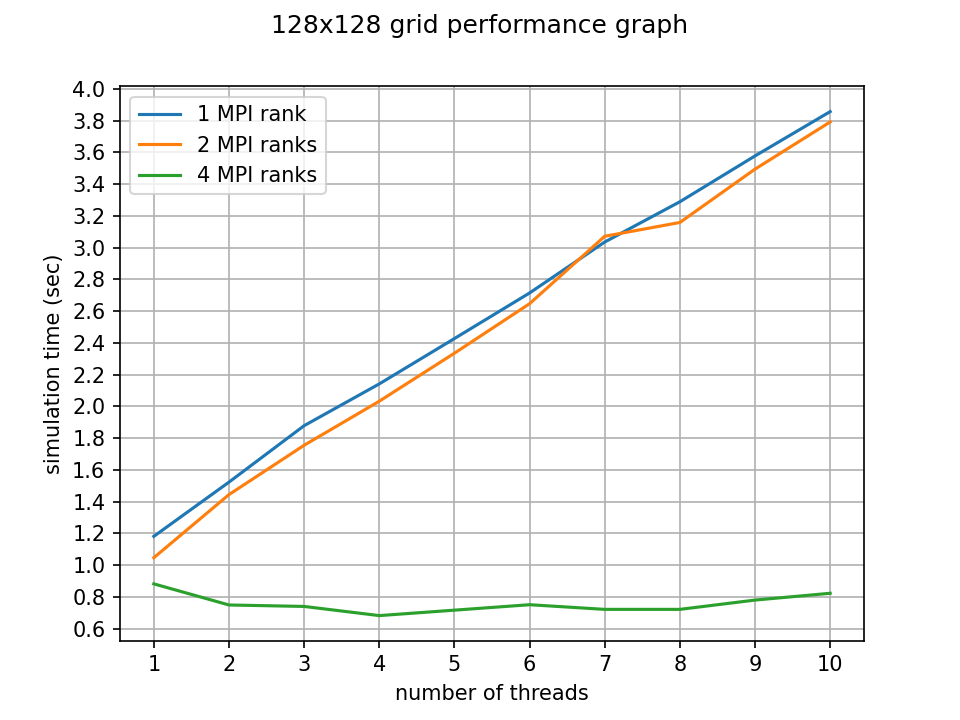
\includegraphics[width=0.9\linewidth]{128x128_plot.png}
\caption{performance graph of the testing done on a 128 by 128 matrix}
\end{figure}

\begin{figure}[H]
\centering
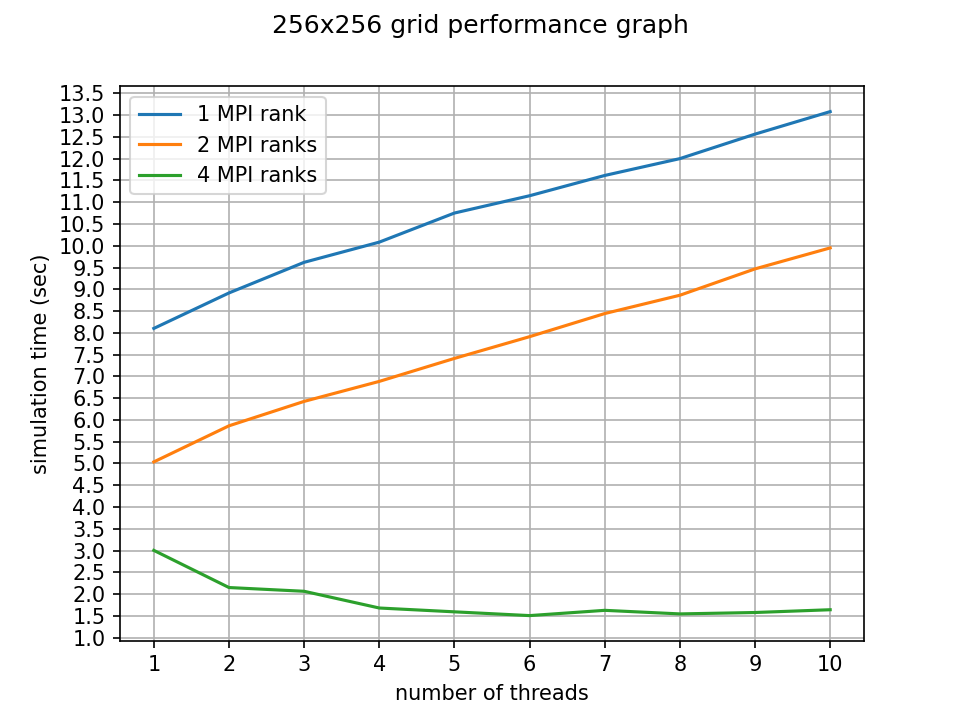
\includegraphics[width=0.9\linewidth]{256x256_plot.png}
\caption{performance graph of the testing done on a 256 by 256 matrix}
\end{figure}

\begin{figure}[H]
\centering
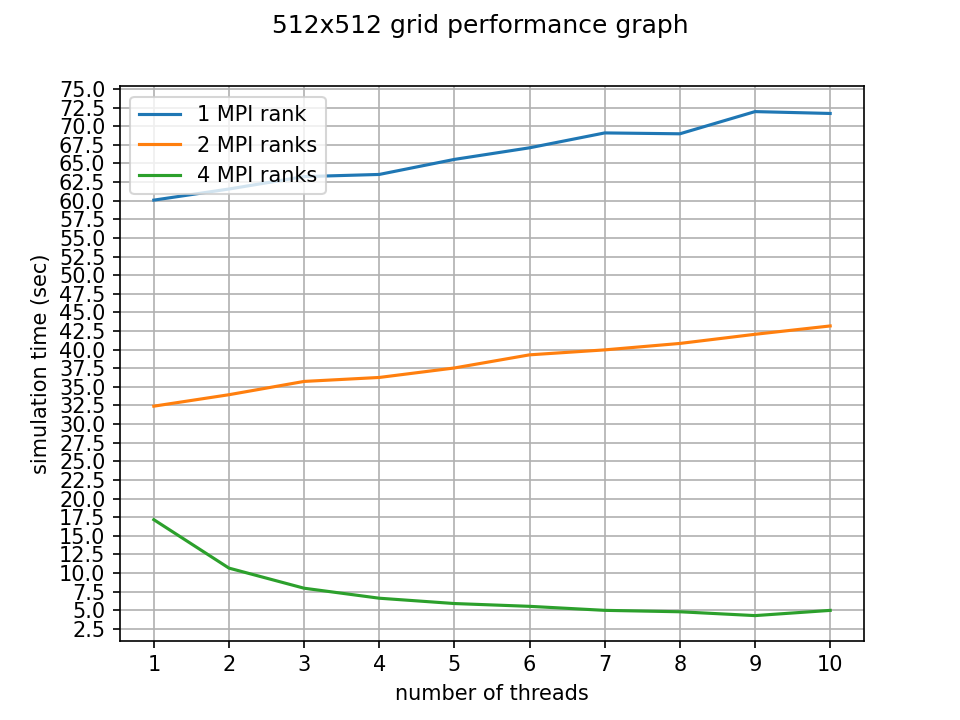
\includegraphics[width=0.9\linewidth]{512x512_plot.png}
\caption{performance graph of the testing done on a 512 by 512 matrix}
\end{figure}

\begin{figure}[H]
\centering
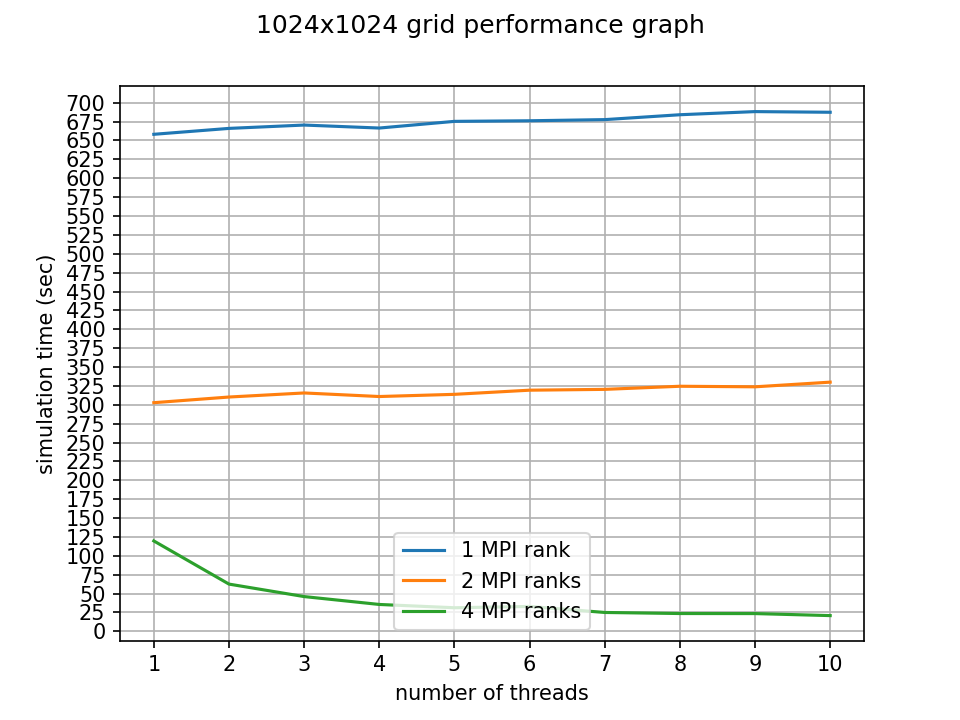
\includegraphics[width=0.9\linewidth]{1024x1024_plot.png}
\caption{performance graph of the testing done on a 1024 by 1024 matrix}
\end{figure}
Some observations:
\begin{itemize}
\item Increasing the number of MPI ranks always improves performance: The bigger the matrix, the bigger the difference between them. Starting from the 256 by 256 matrix, doubling the amount of MPI ranks also doubles the performance.
\item Increasing the number of threads always worsens performance when using 1 or 2 MPI ranks. However, the loss in performance gets smaller as the matrix size increases: it's possible that with higher matrices than the ones tested, performance could improve with more threads.
\item Increasing the number of threads improves performance when using 4 MPI ranks: in the 128 by 128 matrix the best results were had when using 4 threads, in the 256 by 256 one when using 6,  in the 512 by 512 when using 9, and in the 1024 by 1024 when using 10 (the increase in performance also looks logarithmic starting from the 256 by 256 matrix).
\end{itemize}

\section{Task 6 - Quality of the Report [15 Points]}



\end{document}
